\documentclass[12pt,a4paper]{scrartcl}
% scrartcl ist eine abgeleitete Artikel-Klasse im Koma-Skript
% zur Kontrolle des Umbruchs Klassenoption draft verwenden


% die folgenden Packete erlauben den Gebrauch von Umlauten und ß
% in der Latex Datei
\usepackage[utf8]{inputenc}
% \usepackage[latin1]{inputenc} %  Alternativ unter Windows
\usepackage[T1]{fontenc}
\usepackage[ngerman]{babel}


\usepackage[pdftex]{graphicx}
\usepackage{latexsym}
\usepackage{amsmath,amssymb,amsthm}

\usepackage{caption}
\usepackage{subcaption}
\usepackage{pgfplots}
\usepackage{centernot}
\usepackage{tabularx}

% Abstand obere Blattkante zur Kopfzeile ist 2.54cm - 15mm
\setlength{\topmargin}{-15mm}

\begin{document}
\pagestyle{empty}

\begin{titlepage}
\begin{center}
\noindent {\Large Semesterprojekt: Dialoge mit Computern} \\
\vspace{5cm}
\noindent {\Huge Dokumentation zu dem Softwareprodukt Bibo - der freundliche Bibliotheksbot} \\
\vspace{11cm}
\noindent {Iryna Repinetska 562366, Chris Roeseler 561614} \\
\vspace{1cm}
\noindent {Institut f\"ur Informatik \\
		 Humboldt-Universit\"at zu Berlin} \\
\end{center}
\end{titlepage}


\newpage
\tableofcontents
\newpage

\section{Ziele des Projektes}
\begin{itemize}
\item Das Kennenlernen moderner Methoden und Werkzeugen, die es ermöglichen, einen Dialog mit dem Chatbot zu führen, der die Benutzung eines Softwareproduktes für seine Kunden erleichtert.
\item Die Implimentation eines Chatbots, welcher dem Benutzer den Umgang mit der Bibliothek, im Speziellen Auswahl und Ausleihe, erleichtern soll.\\
\item Der Schwerpunkt der Implementation dieses Chatbotes wurde dabei auf drei Aspekte gelegt, die Effektivität der Suche, die Sprachnatürlichkeit und das robuste Verhalten gegen den falschen bzw. nicht erkannten Eingaben.
\end{itemize}
\newpage
\section{Anforderungsanalyse}
\begin{itemize}
\item \textbf{Zielsetzung:}

\begin{enumerate}

\item Mußkriterien:
	\begin{itemize}
		\item Suchparameter des Benutzer abfragen.
		\item Bücher entsprechend der vom Benutzer eingegebenen Parameter finden.
		\item Information über die gesuchte Literatur dem Benutzer vorzustellen.
		\item Eine vom Benutzer ausgewählte Bücherliste nach dem Wunsch per E-mail zu verschicken.
	\end{itemize}
	
\item Wunschkriterien:
	\begin{itemize}
		\item mit möglichst wenigen Schritten Suchattribute abzufragen.
		\item Dialogstruktur der Menschlichen Kommunikation anpassen.
		\item Richtiges Ergebnis trotz unpassenden Antworten des Chatbots, sowie unerkannter Benutzereingaben zu gewährleisten.
	\end{itemize}
	
\item Abgrenzungskriterien: 
	\begin{itemize}
		\item der Bot merkt sich nach dem Ende eines Dialoges, die einem Benutzer zugehörige Parameter nicht.
	\end{itemize}
\end{enumerate}

\end{itemize}




\begin{itemize}
\item \textbf{Produkteinsatz:}

\begin{enumerate}
	\item Anwendungsbereich: das Produkt dient der Auswahl und der Ausleihe der Literatursammlung der HU Bibliothek.
\item Zielgruppen: Die Benutzer der HU Bibliothek (Studenten, Mitarbeiter der Universität).
\end{enumerate}
 
\item \textbf{Produktfunktion:} 
\begin{itemize}
\item Name des Anwendungsszenarios: ein Buch bzw. mehrere Bücher suchen.
\item Kategorie: primär
\item Vorbedingung: -
\item Nachbedingung Erfolg: ein Benutzer bekommt eine Antwort auf seine Anfrage.
\item Nachbedingung Fehlschlag: es gibt keine passende Literatur in der Bibliotheksammlung. Ein Benutzer kann eine neue Anfrage sofort starten.
\item Akteure: ein Benutzer.
\item Auslösendes Ereignis: ein Benutzer schreibt eine Nachricht an den Bot.
\item Beschreibung: die Suchparameter abzufragen; ein Suchergebnis auszugeben.
\item Erweiterung: einen Namen bzw. eine E-Mail-Adresse des Benutzers nachzufragen, die von dem Benutzer ausgewählte Liste an seine E-Mail-Adresse zu verschicken.
	\end{itemize}
\end{itemize}


\begin{itemize}
\item \textbf{Produktdaten:}
\begin{enumerate}
\item Benutzerdaten: ggf. einen Namen und eine E-Mail-Adresse eines Benutzers.
\item Suchparameter:
\begin{itemize}
\item Fall 1: ein Schlüsselwort.
\item Fall 2: einen Titel und ggf. einen Author, einen co-Author, einen Verlag, ein Erscheinungsjahr, ISSN, ISBN oder eine Signatur.
\end{itemize}
\end{enumerate}
\item \textbf{Qualitätsanforderungen:} die qualitativen Eigenschaften des Chatbotes mit den angestrebten Parametern, die für Evaluation des Produktes 'Bibo' im Mittelpunkt gestellt werden, sind in der folgenden Tabelle dargestellt.

\begin{center}
\begin{tabular}{| l| c c c c |}
\hline
Produktqualität & sehr gut & gut & normal & nicht relevant  \\ 
\hline
\textit{Funktionalität}& & & &\\  
Angemessenheit &  &  & $\times$&\\ 
Richtigkeit &  &$\times$  & &\\  
\hline
\textit{Zuverläsigkeit}  &  &  & &\\ 
Fehlertoleranz & $\times$ &  & &\\ 

\hline
\textit{Benutzbarkeit} &  &  & &\\ 
Verständlichkeit &$\times$  &  & &\\ 
Bedienbarkeit & $\times$ &  & &\\ 
Attraktivität & $\times$ &  & &\\ 
\hline
\textit{Effizienz}  &  &  & &\\ 
Zeitverhalten &$\times$   &  & &\\ 
\hline
\end{tabular}
\end{center}

\item \textbf{Systemanforderunen:} eine laufende Internetverbindung.
\end{itemize}
\newpage
\section{Dialogkonzepte}
Ein Dialog zwischen dem Bot und dem Benutzer wird durch das folgende Aktivitätsdiagramm dargestellt.\\
\begin{figure}[h]
\centering
  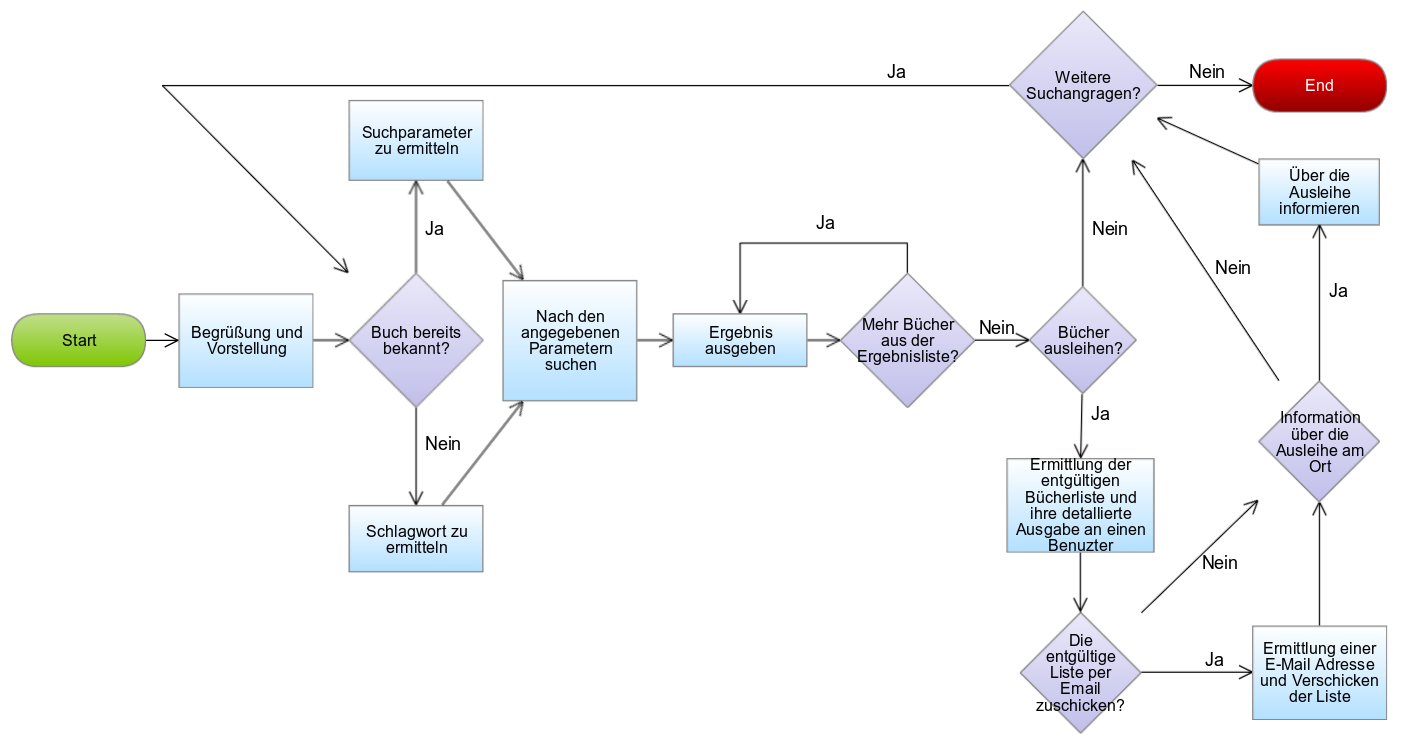
\includegraphics[width=\linewidth]{presbibo1.png}
  \caption{Dialogablauf des Bots dargestellt durch ein Aktivitätsdiagramm.}
\end{figure}
\\
Zu den grundlegenden Schritten eines Dialoges gehören:
\begin{enumerate}
	\item \textit{Begrüßung und Vorstellung:} Wenn ein Benutzer das Programm startet, begrüßt der Bot den Benutzer, und fragt nach seinem Namen. Der Benutzer kann nach Wunsch seinen Namen nicht mitteilen.
	\item \textit{Parametern der Suchanfrage ermitteln:} Ein Buch besitzt mehrere Felder, die dieses Buch in dem Bibliothekskatalog beschreiben. Es werden zwei Fällen unterschieden, wenn ein Benutzer eine gute Vorstellung hat, welches Buch er braucht, oder wenn er nach einem Thema bzw. Schlüsselwort sucht. Im ersten Fall wird ein Benutzer gefragt, den Namen eines Buches anzugeben und wunschgemäß den Autornamen sowie eines von den Attributen (co-Autor, Verlag, Erscheinungsjahr, ISSN, ISBN, Signatur) mitzuteilen. Das Buch wird dabei in die Ergebnisliste mitgenommen, wenn alle von dem Benutzer gesetzte Parameter in den entsprechenden Attributen eines Buches vorhanden sind. Im anderen Fall sollte ein Benutzer nur ein Schlagwort angeben. Dabei wird jedes Buch als passend für die gestellte Anfrage betrachtet, wenn mindestens eines der Buchattributen das angegebene Schlagwort besitzt.
	\item \textit{Ausgabe des Suchergebnisses:} Um einen Benutzer mit der Größe der Ergebnisliste nicht zu überwältigen, wird die Ergebnisliste jeweils in zweierpärchen ausgegeben. Ein Benutzer kann für die Ausgabe mehr Bücher in der Liste anfragen, bis diese leer ist. Danach fragt der Bot, ob ein Benutzer den Wunsch besitzt, ein Buch bzw. mehrere Bücher auszuleihen. In dem positiven Fall werden zwei folgende Möglichkeiten vorgestellt. Ein Benutzer gibt die Büchernummern aus der Ergebnisliste an denen er das Interesse hat. Diese endgültige Liste wird anschließend wunschgemäß per E-Mail-Adresse dem Benutzer zugeschickt. Außerdem kann der Bot den Benutzer über den Ausleihvorgang an dem Ort informieren.
\end{enumerate}
Ein mögliches Szenario einer Interaktion zwischen dem Bot und einem Benutzer wird durch das folgende Sequenzdiagramm dargestellt. Dieses Szenario beschreibt den Fall, wenn ein Benutzer seinen Namen angibt, den Namen des Buches sowie das Erscheinungsjahr kennt, die gesuchte Bücher in der ersten Runde der Ausgabe findet, seine E-Mail-Adresse angibt und keine weiteren Suchanfragen stellt.
\\
\begin{figure}[h!]
 \centering
  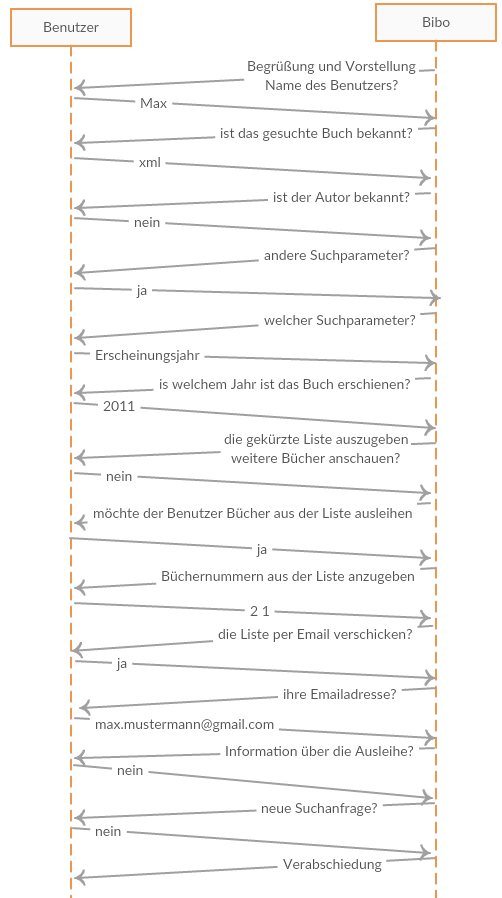
\includegraphics[height= 14 cm]{presbibo2.png}
  \caption{Das Sequenzdiagramm für ein mögliches Gespächsszenario.}
\end{figure}
\newpage
\section{Technische Konzepte}
Der Chatbot 'Bibo' wurde in Python 2.7 geschrieben und baut auf fünf zusätzlichen librarys auf, nämlich aiml, urllib2, BeautifulSoup mit bs4, lxml.                                                Die Architektur des Bots ist in drei Bereiche unterteilt.\\ Bibo.py beinhaltet die Hauptroutine die auf Eingaben des Benutzers reagiert die Buchleihe organisiert und ggf. am Ende des Ablaufs per mail versendet. Nachdem in dieser Hauptroutine ein Dictionary mit der Anfrage des Benutzers erstellt wurde, wird diese an den HTML Parser übergeben.\newline
Dieser ist in url.py und crawl.py               
organisiert. Das parsen des DOM-Baums erfolgt mit BeautifulSoup welches im weiteren mit Bsoup abgekürzt wird. Diese Parser library                                                           
ermöglicht es HTML Elemente aufgrund von Namen, Klassen und Id's zu finden und zu durchsuchen. Wir nutzten lxml als parser. Aus der Anfrage in Dictionary Form wird ein Primolink erstellt der zur                                                                     
jeweiligen HU Bibliotheksseite korrespondiert. Dieser Link setzt grob sich wie folgt zusammen:\newline
[BASEURL]/[FELD][KEYWORD0]?[FELD][KEYWORD1]? [FELD][KEYWORD2][TAIL]. Dabei lässt sich die ganze Funktionalität des Suchportales innerhalb des Links darstellen.   
Das HTML dieser Ergebnissuche wird mit urllib2 geladen und an Bsoup übergeben. Dieses extrahiert aus den einzelnen Suchergebnissen die Links der Detailseiten des jeweiligen         
Ergebnisses. Für jedes Ergebnis wird nun das HTML der Detailseite mit urllib2 geöffnet und die Informationen wieder mit Bsoup extrahiert und in ein Dictionary gespeichert. Hieraus ergibt sich eine Liste mit Dictionarys, welche einer Liste mit Büchern entspricht. In Bibo.py wird diese Liste weiterhin bearbeitet bis sie per Email an den Benutzer geschickt        
werden kann.\newline
Das parsen der Beutzer Antworten wiederum wird mit aiml organisiert. Es wurde die aiml libary     
von Python genutzt. Die aiml Muster sind im bibo.aiml file organisiert. Aufgrund technischer Eingeschränktheit von Pyaiml musste die Interaktion zwischen dem bibo.py und bibo.aiml mit den Stringsvergleichen der letzten Antworten organisiert werden.\newline
Die Abarbeitung der Benutzereingaben von bibo.aiml ähnelt sich an die Arbeitsweise eines endlichen Automaten. Abhängig von den Benutzerantworten und den momentanen Zustand übergeht der Bot in den nächsten eindeutigen Zustand. Jeder Zustand ist durch eine Menge von erkannten Mustern charakterisierbar. Da es in Pyaiml keine getPredicate() Funktion vorgesehen ist, gibt es nur eine Möglichkeit die in bibo.aiml bei einem Benutzer gesetzten Variablen an bibo.py zu übergeben, nämlich durch eine Antwort des Bots. Dabei muss gesorgt werden, dass eine solche Antwort nicht dem Benutzer gezeigt wird.\newline
\newpage
Die Architektur des Chatbots 'Bibo' wird durch das folgende Komponentendiagramm dargestellt.                                                                                \begin{figure}[h!]
 \centering
  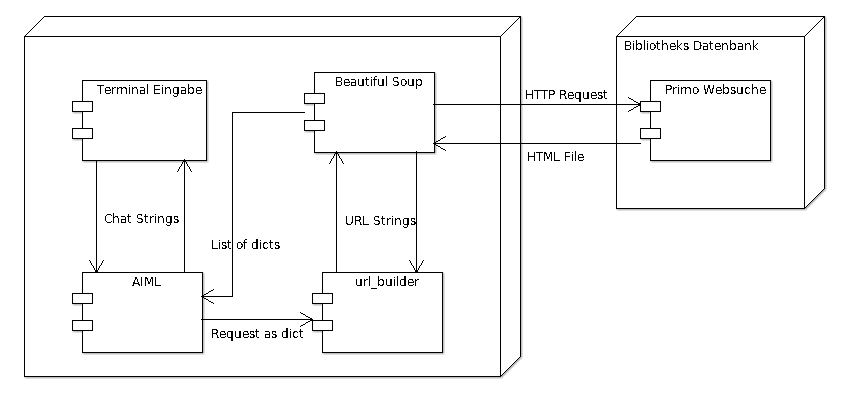
\includegraphics[width=\linewidth]{components.png}
  \caption{Das Komponentendiagramm des Chatbots 'Bibo'.}
\end{figure}
\section{Implimentierungskonzepte}
Die Grundlegende Implementierungsidee von dem Chatbot 'Bibo' ist ein Bot der die Suche im online Portal der Universitätsbibliothek für den Benutzer übernimmt und alles wichtigen Informationen der        
Leihe kompakt darstellt. Hierfür muss der Bot wie ein Benutzer das Suchportal nutzen und sich dort seine Informationen besorgen. Da die Bibliothek keine Api bereitstellt, muss diese         
Informationsbeschaffung über einen HTML crawler organisiert werden. Dies macht ihn theoretisch unabhängig vom speziellen Suchportal.\newline
Der Umgang mit dem User wird über AIML gehändelt. AIML bietet die Möglichkeit auf bestimmte Anfragen mit vorgegebenen Inhalten zu antworten. Wildcard Character ermöglichen weiterhin eine Vielzahl von z.B. Begrüßungen auf eine einzige Begrüßung zu reduzieren. Außerdem kann mit AIML mit Topics gearbeitet werden. Es ist also möglich im geringen Umfang mit früher im Gespräch eingebrachten Informationen zu arbeiten.\newline
Es wurde die Programmiersprache python für die Implementation des Bots gewählt. Pathon ist einfach zu lernen, sehr flexibel, erleichtert die Arbeit im Web durch zahlreiche libraries, ermöglicht eine im Vergleich zu anderen Sprachen einfachere Arbeit mit Strings und hat Pyaiml als eine von seinen libraries.
\newline
\section{Evaluation}
\subsection{Konzept}
Der Anspruch der Evaluation orientiert sich an drei Aspekten. Löst der Bot seine Aufgabe effektiv, ist die Kommunikation menschlich nachvollziehbar und wird das richtige Ergebnis erbracht trotz der unerkannten Eingaben bzw. der unpassenden Antworten des Bots.
\subsection{Durchführung}.
Die Evaluation wurde in zwei Runden durchgeführt.
\begin{enumerate}
\item \textbf{die erste Runde} hat in der Sitzung der Veranstaltung 'Dialoge mit Computern' stattgefunden.
\begin{itemize}

\item \textit{Anzahl der Probanten}: 8 Personen.
\item \textit{Zeit der Unterhaltung mit dem Chatbot}: 5 minuten.
\item \textit{erhobene Daten}: Probanden werden gefragt den folgenden Fragebögen auszufüllen\\

\textbf{Sprachnatürlichkeit}
\begin{center}
\begin{tabularx}{\linewidth}{|X|cccccc|c|}

\hline

&1&2&3&4 &5 &6 &k.A \\ \hline
Ich könnte mit einem Menschen kommuniziert haben. & $\bigcirc$ & $\bigcirc$ & $\bigcirc$ & $\bigcirc$  & $\bigcirc$  & $\bigcirc$  &$\bigcirc$ \\ \hline

Das Gespräch verlief natürlich. & $\bigcirc$ & $\bigcirc$ & $\bigcirc$ & $\bigcirc$  & $\bigcirc$  & $\bigcirc$  &$\bigcirc$ \\ \hline

Ich konnte alle Antworten bzw. Fragen verstehen. & $\bigcirc$ & $\bigcirc$ & $\bigcirc$ & $\bigcirc$  & $\bigcirc$  & $\bigcirc$  &$\bigcirc$\\ \hline

Es gab keine unnötigen Fragen.  & $\bigcirc$ & $\bigcirc$ & $\bigcirc$ & $\bigcirc$  & $\bigcirc$  & $\bigcirc$  &$\bigcirc$ \\ \hline


Dialog Ausschnitte haben sich nicht wiederholt. & $\bigcirc$ & $\bigcirc$ & $\bigcirc$ & $\bigcirc$  & $\bigcirc$  & $\bigcirc$  &$\bigcirc$ \\ \hline

Von mir angegebene Informationen wurden im Verlauf des Dialogs nicht vergessen. & $\bigcirc$ & $\bigcirc$ & $\bigcirc$ & $\bigcirc$  & $\bigcirc$  & $\bigcirc$  &$\bigcirc$ \\ \hline
\multicolumn{8}{|c|}{1 zutreffend, 2 eher zutreffend, 3 etwas zutreffend,}\\
\multicolumn{8}{|c|}{4 wenig zutreffend, 5 eher nicht zutreffend, 6 nicht zutreffend} \\ \hline


\end{tabularx}
\end{center}
\newpage
\textbf{Benutzerfreundlichkeit und Effektivität}
\begin{center}
\begin{tabularx}{\linewidth}{|X|cccccc|c|}

\hline
&1&2&3&4 &5 &6 &k.A \\ \hline

Die Funktionsweise war eindeutig. & $\bigcirc$ & $\bigcirc$ & $\bigcirc$ & $\bigcirc$  & $\bigcirc$  & $\bigcirc$  &$\bigcirc$ \\ \hline

Ich hatte keine Schwierigkeiten die gewünschte Literatur zu finden. & $\bigcirc$ & $\bigcirc$ & $\bigcirc$ & $\bigcirc$  & $\bigcirc$  & $\bigcirc$  &$\bigcirc$ \\ \hline

Es hat nicht lange gedauert bis ich die gewünschte Suchergebnisse bekommen habe.& $\bigcirc$ & $\bigcirc$ & $\bigcirc$ & $\bigcirc$  & $\bigcirc$  & $\bigcirc$  &$\bigcirc$ \\ \hline

Die angebotene Funktionalität war ausreichend.& $\bigcirc$ & $\bigcirc$ & $\bigcirc$ & $\bigcirc$  & $\bigcirc$  & $\bigcirc$  &$\bigcirc$ \\ \hline

Es war effektiver Bibo zu nutzen. & $\bigcirc$ & $\bigcirc$ & $\bigcirc$ & $\bigcirc$  & $\bigcirc$  & $\bigcirc$  &$\bigcirc$ \\ \hline

\multicolumn{8}{|c|}{1 zutreffend, 2 eher zutreffend, 3 etwas zutreffend,}\\
\multicolumn{8}{|c|}{4 wenig zutreffend, 5 eher nicht zutreffend, 6 nicht zutreffend} \\ \hline

\end{tabularx}
\end{center}
\textbf{Allgemein}
\begin{center}
\begin{tabularx}{\linewidth}{|X|cccccc|c|}

\hline
&1&2&3&4 &5 &6 &k.A \\ \hline

Ich möchte Bibo für weitere Literatursuchen verwenden. & $\bigcirc$ & $\bigcirc$ & $\bigcirc$ & $\bigcirc$  & $\bigcirc$  & $\bigcirc$  &$\bigcirc$ \\ \hline


Ich denke das Suchportal kann durch Bibo ersetzten werden. & $\bigcirc$ & $\bigcirc$ & $\bigcirc$ & $\bigcirc$  & $\bigcirc$  & $\bigcirc$  &$\bigcirc$ \\ \hline

Alles in allem bewerte ich die Leistung mit der Note.(Zahlen als Schulnoten) & $\bigcirc$ & $\bigcirc$ & $\bigcirc$ & $\bigcirc$  & $\bigcirc$  & $\bigcirc$  &$\bigcirc$ \\ \hline
\multicolumn{8}{|c|}{1 zutreffend, 2 eher zutreffend, 3 etwas zutreffend,}\\
\multicolumn{8}{|c|}{4 wenig zutreffend, 5 eher nicht zutreffend, 6 nicht zutreffend} \\ \hline
\end{tabularx}
\end{center}


\textbf{Freitextkommentare}

\begin{center}
\begin{tabular}{|l|}
\hline
Das hat mir gefallen: \\ \hline
\\
\\
\\ \hline
Das hat mir nicht gefallen: \\ \hline
\\
\\
\\ \hline
Welche weitere konstruktiven Anregungen und Verbesserungsvorschläge haben Sie? \\ \hline
\\
\\ 
\\
\\ \hline

\end{tabular}
\end{center}
\end{itemize}
\item \textbf{die zweite Runde} wurde in der HU-Bibliothek (Jacob-und-Wilhelm-Grimm-Zentrum) druchgeführt.
\begin{itemize}

\item \textit{Anzahl der Probanten}: 20 Personen.
\item \textit{Zeit der Unterhaltung mit dem Chatbot}: 5 minuten.
\item \textit{erhobene Daten}: Probanden werden gefragt erst eine Suchanfrage an den Chatbot 'Bibo' zu stellen und anschließend die gleiche Anfrage mit dem Suchportal zu machen. Danach sollten die Probanden den oben erwähnten Fragebogen ausfüllen.\\ 
\end{itemize}
\end{enumerate}
\subsection{Ergebnisse}
\begin{enumerate}
\item \textbf{erste Evaluation:}
\begin{itemize}
\item \textit{Sprachnatürlichkeit}

\begin{center}
\begin{tabularx}{\linewidth}{|X|r|}
\hline
Gestellte Frage & Durchschnittliche Note  \\ \hline

Ich könnte mit einem Menschen kommuniziert haben. & $2,3$  \\ \hline

Das Gespräch verlief natürlich. & $3$   \\ \hline

Ich konnte alle Antworten bzw. Fragen verstehen. & $3$ \\ \hline

Es gab keine unnötigen Fragen. & $3,75$  \\ \hline


Dialog Ausschnitte haben sich nicht wiederholt. & $3$  \\ \hline

Von mir angegebene Informationen wurden im Verlauf des Dialogs nicht vergessen. & $1,9$  \\ \hline
\multicolumn{2}{|c|}{1 zutreffend, 2 eher nicht zutreffend, 3 etwas zutreffend} \\ \hline
\multicolumn{2}{|c|}{4 wenig zutreffend, 5 eher nicht zutreffend, 6 nicht zutreffend} \\ \hline
\end{tabularx}
\end{center}
\textbf{Insgesamt erhält die Sprachnatürlichkeit die mittlere Note 2,8.}
\item \textit{Benutzerfreundlichkeit und Effektivität}
\begin{center}
\begin{tabularx}{\linewidth}{|X|c|}

\hline
Gestellte Frage & Durchschnittliche Note  \\ \hline
Die Funktionsweise war eindeutig. & $1,3$ \\ \hline

Ich hatte keine Schwierigkeiten die gewünschte Literatur zu finden. & $3,1$\\ \hline

Es hat nicht lange gedauert bis ich die gewünschte Suchergebnisse bekommen habe.& $4$\\ \hline

Die angebotene Funktionalität war ausreichend.& $4$ \\ \hline

Es war effektiver Bibo zu nutzen. & $3,9$ \\ \hline

\multicolumn{2}{|c|}{1 zutreffend, 2 eher zutreffend, 3 etwas zutreffend,}\\
\multicolumn{2}{|c|}{4 wenig zutreffend, 5 eher nicht zutreffend, 6 nicht zutreffend} \\ \hline

\end{tabularx}
\end{center}
\textbf{Insgesamt erhält die Benutzerfreundlichkeit und Effektivität die mittlere Note 3,3.}
\newpage
\item \textit{Allgemein}
\begin{center}
\begin{tabularx}{\linewidth}{|X|c|}

\hline
Gestellte Frage & Durchschnittliche Note  \\ \hline
Ich möchte Bibo für weitere Literatursuchen verwenden. & $3,1$ \\ \hline


Ich denke das Suchportal kann durch Bibo ersetzten werden. & $2$ \\ \hline

Alles in allem bewerte ich die Leistung mit der Note.(Zahlen als Schulnoten) & $3,3$ \\ \hline
\multicolumn{2}{|c|}{1 zutreffend, 2 eher zutreffend, 3 etwas zutreffend,}\\
\multicolumn{2}{|c|}{4 wenig zutreffend, 5 eher nicht zutreffend, 6 nicht zutreffend} \\ \hline
\end{tabularx}
\end{center}
\textbf{Insgesamt erhält die Wiederverwendbarkeit des Produktes die mittlere Note 2,8.}
\item \textit{Kommentate}\newline
Einige der wichtigesten Kommentare waren:
\begin{itemize}
\item der Ablauf ist sehr statisch.
\item ich konnte nicht verstehen, welche Antwort von mit erwartet wird.
\item zu lange, zu viele Schritten bis zum Ergebnis.
\item der Bot zeigt keine neue Funktionalität im Vergleich zu dem Suchportal.
\item lustige, passende Antworten des Botes.
\end{itemize}

\end{itemize}






\item \textbf{zweite Evaluation:}
\begin{itemize}
\item \textit{Sprachnatürlichkeit}

\begin{center}
\begin{tabularx}{\linewidth}{|X|r|}
\hline
Gestellte Frage & Durchschnittliche Note  \\ \hline

Ich könnte mit einem Menschen kommuniziert haben. & $1,8$  \\ \hline

Das Gespräch verlief natürlich. & $2$   \\ \hline

Ich konnte alle Antworten bzw. Fragen verstehen. & $2,3$ \\ \hline

Es gab keine unnötigen Fragen. & $2,5$  \\ \hline


Dialog Ausschnitte haben sich nicht wiederholt. & $2,8$  \\ \hline

Von mir angegebene Informationen wurden im Verlauf des Dialogs nicht vergessen. & $2,1$  \\ \hline
\multicolumn{2}{|c|}{1 zutreffend, 2 eher nicht zutreffend, 3 etwas zutreffend} \\ \hline
\multicolumn{2}{|c|}{4 wenig zutreffend, 5 eher nicht zutreffend, 6 nicht zutreffend} \\ \hline
\end{tabularx}
\end{center}
\textbf{Insgesamt erhält die Sprachnatürlichkeit die mittlere Note 2,3.}
\item \textit{Benutzerfreundlichkeit und Effektivität}
\begin{center}
\begin{tabularx}{\linewidth}{|X|c|}

\hline
Gestellte Frage & Durchschnittliche Note  \\ \hline
Die Funktionsweise war eindeutig. & $1,5$ \\ \hline

Ich hatte keine Schwierigkeiten die gewünschte Literatur zu finden. & $3,0$\\ \hline

Es hat nicht lange gedauert bis ich die gewünschte Suchergebnisse bekommen habe.& $4$\\ \hline

Die angebotene Funktionalität war ausreichend.& $2,3$ \\ \hline

Es war effektiver Bibo zu nutzen. & $2,8$ \\ \hline

\multicolumn{2}{|c|}{1 zutreffend, 2 eher zutreffend, 3 etwas zutreffend,}\\
\multicolumn{2}{|c|}{4 wenig zutreffend, 5 eher nicht zutreffend, 6 nicht zutreffend} \\ \hline

\end{tabularx}
\end{center}
\textbf{Insgesamt erhält die Benutzerfreundlichkeit und Effektivität die mittlere Note 2,7.}

\item \textit{Allgemein}
\begin{center}
\begin{tabularx}{\linewidth}{|X|c|}

\hline
Gestellte Frage & Durchschnittliche Note  \\ \hline
Ich möchte Bibo für weitere Literatursuchen verwenden. & $2,1$ \\ \hline


Ich denke das Suchportal kann durch Bibo ersetzten werden. & $2$ \\ \hline

Alles in allem bewerte ich die Leistung mit der Note.(Zahlen als Schulnoten) & $2$ \\ \hline
\multicolumn{2}{|c|}{1 zutreffend, 2 eher zutreffend, 3 etwas zutreffend,}\\
\multicolumn{2}{|c|}{4 wenig zutreffend, 5 eher nicht zutreffend, 6 nicht zutreffend} \\ \hline
\end{tabularx}
\end{center}
\textbf{Insgesamt erhält die Wiederverwendbarkeit des produktes die mittlere Note 2,0.}
\item \textit{Kommentate}
Einige der wichtigesten Kommentare waren:
\begin{itemize}
\item es dauert zu lange bis zum Ergebnis.
\item natürliche Sprache.
\end{itemize}
\end{itemize}
\end{enumerate}

\subsection{Analyse}
Nach der ersten Evaluation wurde der Chatbot mit der mittleren Note 3 bewertet. Dir größten Schwächen des Bots waren die lange Laufzeit, keine Erkennung von Sätzen als Eingaben, nicht genügende Funktionalität des Bots.\newline
Um die allgemeine Zufriedenheit mit 'Bibo' zu verbessern, haben wir versucht in den nächsten drei Wochen  die oben erwähnten Probleme zu beheben bzw. mildern.\newline
Die zweite Evaluation hat die Verbesserung der Bewertungen um ungefähr 0,6 Punkte gezeigt. 
\section{Fazit}
\begin{itemize}
\item \textit{die Stärken des Botes: }\newline
Der Bot liefert vorwiegend ein robustes Verhalten gegen den unerkannten Eingaben des Benutzers. Außerdem wurde die Botantworten als menschlich, natürlich und größtenteils passend angesehen. Der Bot ist in der Lage in meisten Fällen eine an ihn gestellte Suchanfrage in wenigen Schritten so zu beantworten, dass es einen Benutzer zufrieden stellt. 
\item \textit{die Schwächen des Botes: }
\begin{itemize}
\item der Bot ist nicht in der Lage an vielen Stellen die vollen Sätze zu verstehen.
\item das Gespräch ist mit ggf. unnötigen Ja/Nein-Fragen belastet.
\item es dauert lange von dem Moment wenn alle Suchparameter ermittelt werden bis zur Ausgabe der gefundenen Bücher.
\end{itemize}
\item \textit{die während der Implementation aufgetretene Probleme.} \newline
Während der Implementation des Bots kam es zu mehreren Problemen. Die Erzeugung des Links und das crawlen der einzelnen Seiten bietet einige Probleme. So wurde während des Entwicklungsprozesses die HTML Struktur des Suchportals umgestellt, welche zur Folge hat das der crawler deutlich schwerer an die einzelnen Ergebnisse kommt. Nach öffnen des ersten Links müssen für jedes weitere Ergebnis zweite http Anfragen gestellt werden. Außerdem scheint das Primo Portal auf automatisierte Anfragen schlecht zu reagieren, da nur bei ca jedem dritten Versuch das
gewünscht HTML erscheint. Dieser Overhead sorgt für eine sehr schlechte Laufzeit des crawlers und bietet viel Angriffsfläche für Bugs die aus der Umstellung des Suchportales hervorgehen. Nicht zuletzt ist auch die Bibliothek selbst mit Fehlern versehen. Wie oft bei solch großen Datenbanken sind nicht alle Einträge korrekt nach Konvention erstellt und erschweren die Arbeit des crawlers enorm. Um diesen Problemen entgegenzuwirken wurde entschieden die Menge der Suchergebnisse auf 10 zu begrenzen.\newline
Außerdem sind wir im Laufe der Produktentwicklung auf das Problem der funktionalen Begrenztheit von Pyaiml gestoßen. Es hat sich z. B. herausgestellt, dass eine Eingabe die einen Punkt bereithält als zwei verschiedene Eingaben erkannt wird, falls eine Wildcard am Anfang des Musters steht, dann wird es als ein Muster mit nur einer Wildcard verstanden, unabhängig davon, ob es nach dieser Wildcard noch weitere Wörter stehen. Wie oben bereits erwähnt wurde, gibt es keine Funktion, die in der Lage ist, die im .aiml-Teil gesetzten Variablen an den .py-Teil zu übergeben. Deswegen wird das Zusammenspiel zwischen diesen Teilen nur durch die Antworten des Botes bzw. Eingaben an .aiml-Teil beschränkt. Das alles führt dazu, dass es unmöglich ist, einen Chatbot so zu implementieren, dass die ganze Sätze verstanden werden und gleichzeitig bei den unerkannten Eingaben das richtige Ergebnis geliefert wird.
\end{itemize}
\section{Link auf das Produkt}
https://github.com/chroeseler/bibo/tree/master/src
\end{document}
